\section{Расчёт критических кумулянтов для модели прямоугольного Изинга}

Кумулянт Биндера для модели Изинга в критической точке расчитывается по формуле:
\begin{equation}
\label{eq:Cumulant}
U_{4} = 1 - \frac{\la m^{4} \ra}{3 * (m^{2})^{2}}
\end{equation}

где $\la m^{2} \ra$ - средний квадрат удельной намагниченности, $\la m^{4} \ra$ - средная удельная намагниченность в четвертой степени. 

Для сравнения значения кумулянтов модели прямоугольного Изинга с разными размерами, но одинаковым отношением сторон (так же Aspect Ratio), были проведены симуляции модели на основе алгоритма из проектной работы Сорокина Никиты \cite{Schro} и Камиллы Файзулиной \cite{SAW} - для этого были взяты длины 50, 100, 200 и 400 и отношения сторон 1/4, 1/2, 3/4 при $2 * 10^{6}$ итераций.

\begin{figure}[!h]
    \centering
    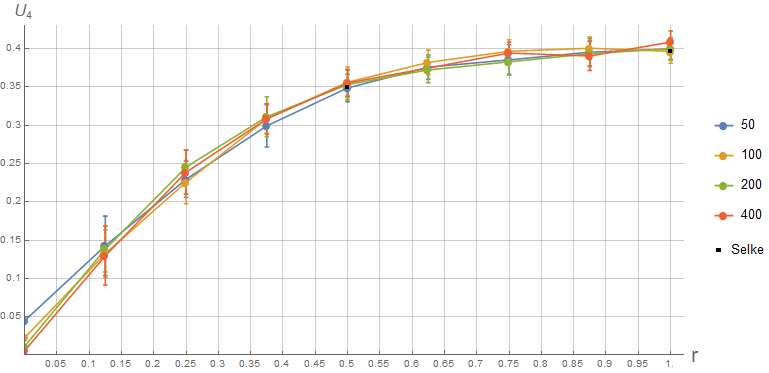
\includegraphics[width=150mm]{Sections/Images/CumulantOBC.png}
    \label{fig:CumulOBC}
    \caption{График зависимости значения кумулянта Биндера в крит. точке от Aspect Ratio при открытых гран. условиях}
\end{figure}

\begin{figure}[!h]
    \centering
    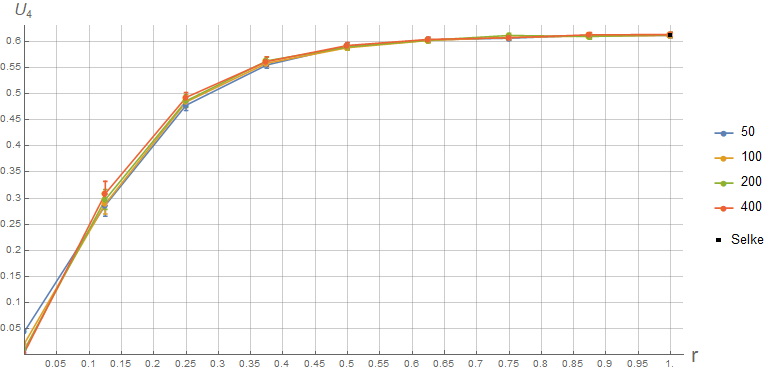
\includegraphics[width=150mm]{Sections/Images/CumulantPBC.png}
    \label{fig:CumulOBC}
    \caption{График зависимости значения кумулянта Биндера в крит. точке от Aspect Ratio при периодических гран. условиях}
\end{figure}